\section{Tekstanalyse}
\subsection{Sensor}
	\begin{description}[style=nextline]
		\item[Kan vi få fat i data?]
		På Android kan man få adgang til SMS beskeder. Hvor tankegangen er at disse analyseres til at finde ud af en persons sindsstemning.
		\item[Er der begrænsninger]
		Hvis man i manifestet skal have rettighed til at læse SMS'er er der ikke begrænsninger.
		Dog er der spørgsmålet om privatliv der skal overvejes.
		\item[Hvilke data gives der?]
		Sms beskeder, d.v.s. en mængde af ustrukturerede tekster med tilknyttet metadata, såsom afsendelsestidspunkt og modtager.
	\end{description}
	
\subsection{Analyse}
	\begin{description}[style=nextline]
		\item[Har vi data nok?]
		Hvis man skal lave sentiment analysis kræver det en stor mængde af træningsdata, for at tekstanalysen bliver akkurat. Twitter kunne evt. være en ressource til at finde sådanne data. Problemet er at det skal være på dansk, og er nok her en stor del af arbejdet med sentiment analysis af danske SMS tekster ligger.
		\item[Hvilke data skal benyttes?]
		Selve SMS teksterne vil være centrale i tekstanalyse til at blive analyseret på.
		Dog kan andre metadata såsom afsendelsestidspunkt, modtager, længde, og respons måske også være interessante at kigge på, og kan også nemt udtrækkes \citep{misc:androidsmsread}.
		
		Afsendelsestidspunkt kunne e.v.t. være interessant til at se om sindstilstand er kontinuert, således at man kan se om en negativ ladet sms tekst er vedvarende over en længere periode eller om det er et enkeltstående tilfælde.
		
		Modtager kunne være interessant til at se om man til personer man normalt har en ensformig tekst stemning mod ændrer sig til eksempelvis meget negativt ladede tekster.
		
		Længden af SMSerne kan eksempelvis bruges til at registere adfærdsændringer, eksempelvis en person der typisk har SMS'er med en længde på 10 ord i gennemsnit pludselig får et gennemsnit på 30+ ord.
		
		Respons kan bruges til at begrunde hvorfor man har et givent toneleje i sine SMS'er. baseret på tonelejet af de SMS'er der svares på.
		\item[Formål med analysen]
		At kunne få en indikation på en persons sindstilstand.
		\item[Idé til visualisering]
		For et øjebliksbillede kunne man give en beskrivende besked om ens sindstilstand, evt. med et tal for hvor sikker vi er på denne bedømmelse.
		Vi forestiller os her en skala over sindstilstande, hvor forskellige niveauer har en dertilhørende beskrivelse.
		Hvis man skulle tage analysen i et kronologisk perspektiv kunne en graf med tid på abscisse aksen og sindstilstandsniveau på ordinat aksen være en mulighed.
		\item[Oprids a fremgangsmåde]
		Udfra træningsdata opbyg en sentiment analysis classifier, eksempelvis Naive Bayes classifier.
		Brug denne classifier til at vurdere sindstilstand for personer, vi forestiller os dette som et modul der kan integreres med andre måder at vurdere en persons sindstilstand.
	\end{description}
	
	\begin{figure}
		\centering
		\begin{subfigure}[b]{0.4\textwidth}
			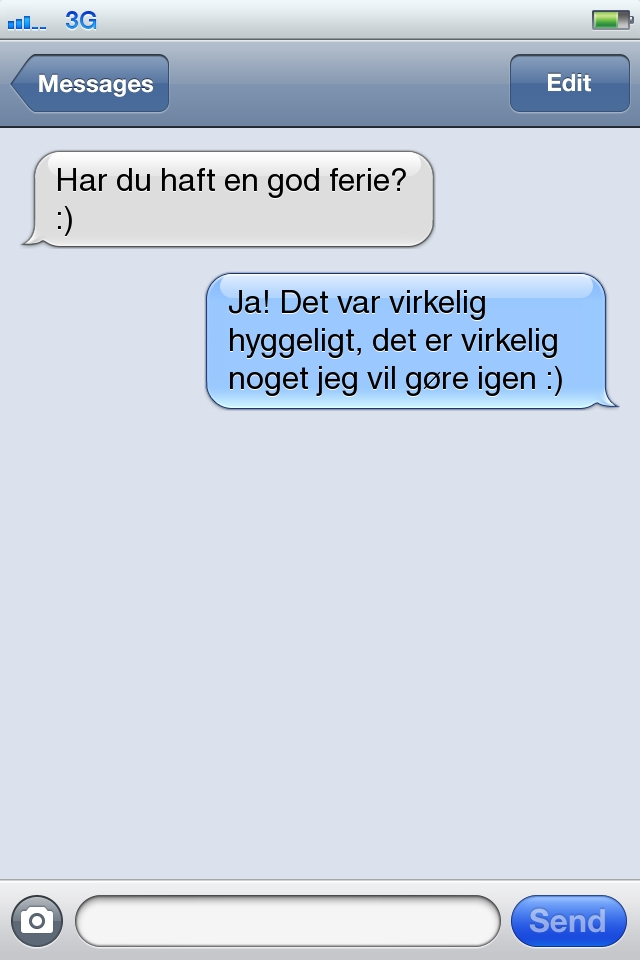
\includegraphics[width=\textwidth]{positiveSMS}
			\caption{Positiv SMS}
		\end{subfigure}
		~
		\begin{subfigure}[b]{0.4\textwidth}
			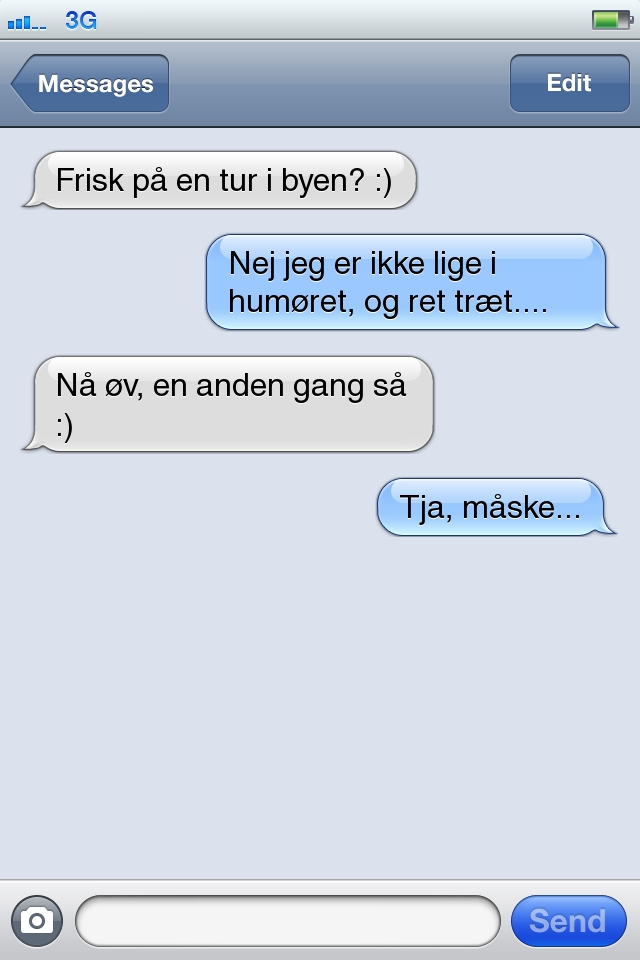
\includegraphics[width=\textwidth]{negativeSMS}
			\caption{Negativ SMS}
		\end{subfigure}
		\caption{Eksempler på SMS'er}
	\end{figure}